% ============================== V. EXPERIMENTS AND RESULTS ==============================
% Số liệu đã đo lấy từ run 20261016-055308_oracle_mediapipe_gemini_rag-report-2t (oracle + eval pred),
% outputs/kinect_compare_U001_V001.json và `python -m kaizen.train.pose eval` (MediaPipe, U001_V002).
% Ô \tbd = DRAFT, điền sau khi train/đánh giá trên nhiều subject.
\section{Experiments and Results}
\label{sec:exp}

\subsection{Thiết lập thực nghiệm}
\label{subsec:setup}
\textbf{Dữ liệu.} Kết quả ở mục này được đo trên U001\_V001 và U001\_V002 của HA4M.
Thực nghiệm huấn luyện dùng \todo{tập subject, cách chia train/val/test hoặc LOSO}.
\textbf{Phần cứng.} \todo{CPU (số lõi), RAM, GPU nếu có}. Mọi bước suy luận trong bài chạy trên CPU.
\textbf{Chỉ số.}
\begin{itemize}
  \item Pose: sai số pixel so với skeleton Kinect (trung vị, P90, tỷ lệ frame lệch $<50$\,px) và PCK@$\alpha$.
        PCK@$\alpha$ là tỷ lệ khớp có sai số $<\alpha$ lần cạnh dài của khung người.
  \item Phân đoạn bước: \Fone, MAE thời lượng bước, MAE mốc bắt đầu và kết thúc, sai số cycle time.
        Với MS-TCN báo thêm độ chính xác frame, Edit và F1@\{10,25,50\} \cite{farha2019mstcn}.
  \item LLM: tỷ lệ đạt validator ngay lần đầu và sau khi hỏi lại.
\end{itemize}

\subsection{Độ chính xác ước lượng cổ tay}
\label{subsec:exp_pose}
Bảng~\ref{tab:kinect} so sánh cổ tay MediaPipe với skeleton Kinect đã chiếu lên ảnh Color.
Lưu ý rằng skeleton Kinect cũng là một ước lượng.
Tay phải bám tốt: trung vị 24{,}5\,px và 95{,}1\% frame lệch dưới 50\,px, tức nhỏ hơn kích thước một khay trên ảnh $2048\times1536$.
Tay trái kém tin cậy hơn (P90 151{,}6\,px) vì thường bị thân người và cụm lắp che.
Tỷ lệ phát hiện người đạt 0{,}953 (V001) và 0{,}961 (V002).
Trên U001\_V002, MediaPipe đạt PCK@0{,}05 bằng 58{,}4 và PCK@0{,}1 bằng 77{,}6 (trung bình mọi khớp COCO-17).
Sai số trung vị là 23{,}3\,px ở cổ tay phải và 26{,}6\,px ở cổ tay trái.

\begin{table}[t]
\centering
\caption{Cổ tay MediaPipe so với skeleton Azure Kinect (U001\_V001)}
\label{tab:kinect}
\footnotesize
\begin{adjustbox}{max width=\columnwidth}
\begin{tabular}{@{}lrrrr@{}}
\toprule
Tay & Số frame & Trung vị (px) & P90 (px) & $<$50\,px (\%) \\
\midrule
Trái & 2148 & 26{,}1 & 151{,}6 & 77{,}7 \\
Phải & 2314 & 24{,}5 & 43{,}4 & 95{,}1 \\
\bottomrule
\end{tabular}
\end{adjustbox}
\end{table}

\begin{table}[t]
\centering
\caption{PCK so với Kinect trên người lắp chưa thấy (DRAFT)}
\label{tab:pck}
\footnotesize
\setlength{\tabcolsep}{3pt}
\begin{adjustbox}{max width=\columnwidth}
\begin{tabular}{@{}lcccc@{}}
\toprule
Backend & PCK@0{,}05 & PCK@0{,}1 & L-wrist (px) & R-wrist (px) \\
\midrule
MediaPipe (U001\_V002) & 58{,}4 & 77{,}6 & 26{,}6 & 23{,}3 \\
RTMW-m & \tbd & \tbd & \tbd & \tbd \\
RTMPose-m fine-tune & \tbd & \tbd & \tbd & \tbd \\
\bottomrule
\end{tabular}
\end{adjustbox}
\end{table}

\subsection{Phân đoạn bước}
\label{subsec:exp_seg}
\textbf{Baseline quy tắc.} \Cref{tab:seg} cho kết quả của baseline quy tắc (\cref{alg:rule}) so với nhãn HA4M.
Trên V001, 15/17 đoạn được neo, với \Fone{} 0{,}75, MAE thời lượng 0{,}62\,s và sai số cycle time 0{,}6\,s.
Trên V002, lần lặp thứ ba của bước 3 (3.2) và bước 5 không được neo, nên chỉ có 11/17 đoạn; \Fone{} đạt 0{,}714 và sai số cycle time 2{,}27\,s.
Phân tích lỗi cho thấy ba nguồn chính:
\begin{enumerate}
  \item bước 9 không có khay đặc trưng nên không có mốc;
  \item mốc bắt đầu bước 10 trễ 4{,}77\,s (V001) và 3{,}13\,s (V002), vì công nhân với tới khay nắp trước khi
        kết thúc thao tác bước 9;
  \item mốc kết thúc bước 12 lệch 2--3{,}5\,s, do bước 12 gồm cả việc trả lục giác và sản phẩm, không có sự kiện neo rõ.
\end{enumerate}
Các bước 1--8 có IoU từ 0{,}43 tới 0{,}80 và độ lệch mốc thường dưới 1\,s.

\begin{table}[t]
\centering
\caption{Phân đoạn bước so với nhãn HA4M. Dòng MS-TCN là DRAFT.}
\label{tab:seg}
\footnotesize
\setlength{\tabcolsep}{2.5pt}
\begin{adjustbox}{max width=\columnwidth}
\begin{tabular}{@{}llcccccc@{}}
\toprule
Phương pháp & Trial & Bước & \Fone & MAE dur & MAE start & MAE end & $\lvert\Delta$CT$\rvert$ \\
            &       & neo/nhãn & & (s) & (s) & (s) & (s) \\
\midrule
Rule & V001 & 15/17 & 0{,}750 & 0{,}62 & 1{,}11 & 0{,}87 & 0{,}60 \\
Rule & V002 & 11/17 & 0{,}714 & 0{,}92 & 0{,}80 & 1{,}05 & 2{,}27 \\
\midrule
MS-TCN (LOSO) & \tbd & \tbd & \tbd & \tbd & \tbd & \tbd & \tbd \\
MS-TCN (test) & \tbd & \tbd & \tbd & \tbd & \tbd & \tbd & \tbd \\
\bottomrule
\end{tabular}
\end{adjustbox}
\end{table}

\textbf{MS-TCN (DRAFT).}
\Cref{tab:mstcn} được điền từ đầu ra của \code{segmenter cv} và \code{segmenter eval}.
\todo{Nhận xét: MS-TCN có tách được bước 9 (không khay) và sửa mốc bước 10, 12 hay không;
so sánh \Fone{} với baseline 0{,}75/0{,}714; phân mảnh đoạn (Edit) trước và sau khi làm mượt.}

\begin{table}[t]
\centering
\caption{MS-TCN, chỉ số chuẩn phân đoạn hành động (DRAFT)}
\label{tab:mstcn}
\footnotesize
\setlength{\tabcolsep}{3pt}
\begin{adjustbox}{max width=\columnwidth}
\begin{tabular}{@{}lccccc@{}}
\toprule
Thiết lập & Acc & Edit & F1@10 & F1@25 & F1@50 \\
\midrule
LOSO, \tbd{} người & \tbd & \tbd & \tbd & \tbd & \tbd \\
Test giữ riêng & \tbd & \tbd & \tbd & \tbd & \tbd \\
Ablation: không $\mathcal{L}_{T\text{-}MSE}$ & \tbd & \tbd & \tbd & \tbd & \tbd \\
Ablation: $S=1$ stage & \tbd & \tbd & \tbd & \tbd & \tbd \\
Ablation: chỉ toạ độ theo thân & \tbd & \tbd & \tbd & \tbd & \tbd \\
\bottomrule
\end{tabular}
\end{adjustbox}
\end{table}

\begin{figure}[t]
  \centering
  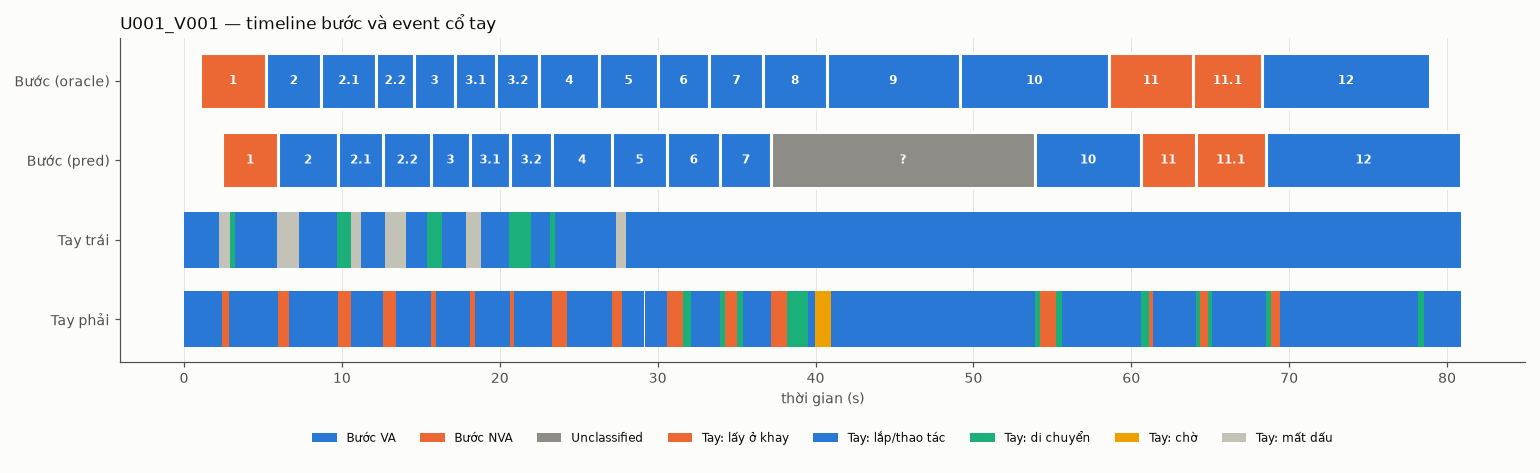
\includegraphics[width=0.9\textwidth]{gantt_U001_V001.png}\\[4pt]
  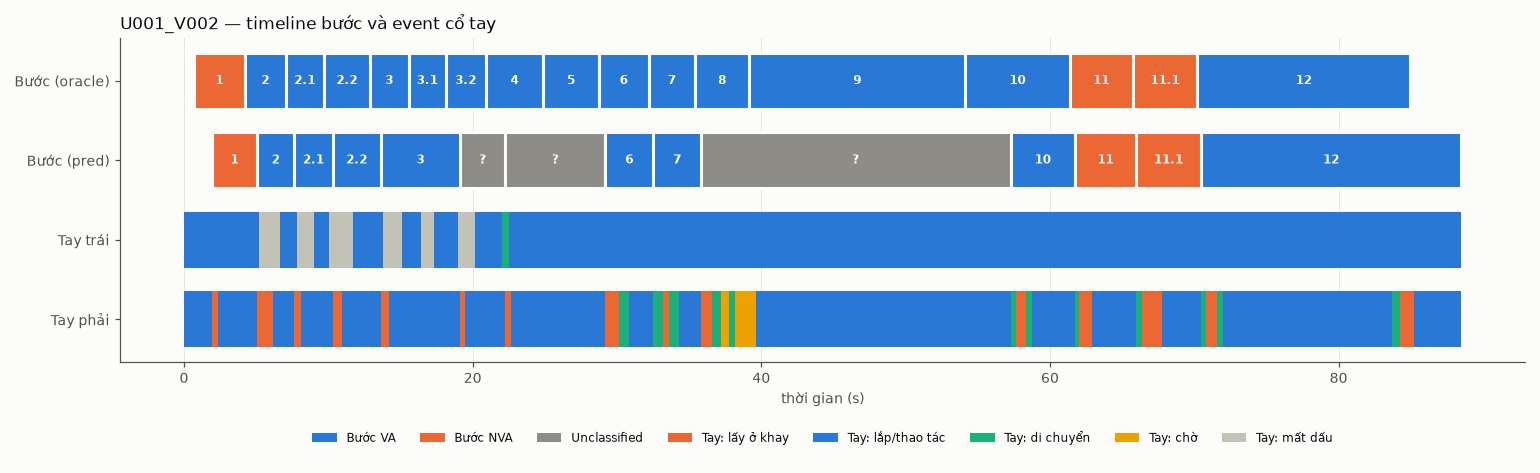
\includegraphics[width=0.9\textwidth]{gantt_U001_V002.png}
  \caption{Timeline Gantt các bước: nhãn HA4M (oracle) so với dự đoán bằng quy tắc, U001\_V001 (trên) và U001\_V002 (dưới).}
  \label{fig:gantt}
\end{figure}

\subsection{Chỉ số Kaizen và phát hiện: nghiên cứu tình huống}
\label{subsec:exp_case}
Ở chế độ oracle, cycle time là 77{,}9\,s (V001) và 84{,}3\,s (V002).
Trung bình là 81{,}1\,s với CV 0{,}056, dưới ngưỡng R6 (0{,}25).
\%VA đạt 82{,}1\% và 85{,}3\%.
Số lần lấy là 15 và 14.
Quãng đường cổ tay trái và phải là 18\,660 và 13\,715\,px (V001).
\Cref{fig:yamazumi} cho thấy thời lượng bước khá ổn định giữa hai lần lắp, trừ bước 9 (CV 0{,}395) và bước 12 (CV 0{,}231).

So với thời gian chuẩn trong work instruction, V001 nằm trong ngưỡng $\pm30\%$ ở mọi bước (lệch từ $-4{,}8\%$ tới $+5{,}0\%$).
V002 kích hoạt hai phát hiện R8:
\begin{itemize}
  \item bước 9 mất 14{,}97\,s so với chuẩn 8{,}5\,s ($+76{,}1\%$; ảnh hưởng 6{,}47\,s/chu kỳ);
  \item bước 12 mất 14{,}77\,s so với chuẩn 11\,s ($+34{,}3\%$; 3{,}77\,s/chu kỳ).
\end{itemize}
R2 phát hiện thêm một lần lấy dư ở khay vít/lục giác (0{,}78\,s/chu kỳ).
Tổng tiềm năng cải thiện là 5{,}5\,s/chu kỳ, tính bằng cộng thô ảnh hưởng của các phát hiện, chưa khử trùng lặp.
Về Muri (\cref{tab:muri}), tay phải được đo trên gần 90\% frame và lệch $>30^\circ$ trong 11{,}5--15{,}2\% thời gian.
Tay trái chỉ đo được khoảng 25\% frame vì điểm bàn tay hay mất. Vì vậy R7 chỉ đánh giá độ tin cậy \textit{low}
và báo kèm độ phủ.
R1 bị bỏ qua vì cần ít nhất 3 trial; R4 ở chế độ oracle xác nhận chuỗi nhãn khớp SOP 12 bước.

\begin{figure}[t]
  \centering
  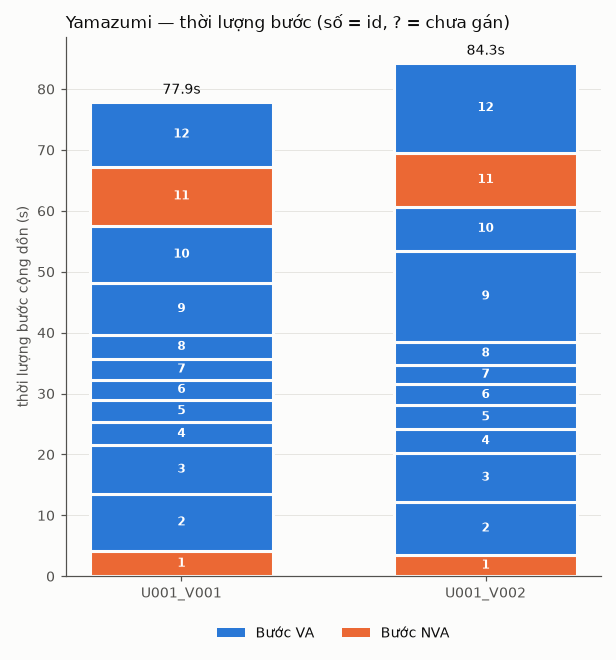
\includegraphics[width=0.8\textwidth]{yamazumi.png}
  \caption{Biểu đồ Yamazumi: thời lượng các bước chồng theo trial (oracle).}
  \label{fig:yamazumi}
\end{figure}

\begin{table}[t]
\centering
\caption{Muri: góc cổ tay 2D (sàng lọc)}
\label{tab:muri}
\footnotesize
\setlength{\tabcolsep}{3pt}
\begin{adjustbox}{max width=\columnwidth}
\begin{tabular}{@{}llrrrr@{}}
\toprule
Trial & Tay & Phủ (\%) & Trung vị (°) & $>30^\circ$ (\%) & P90 $\Delta$ (°) \\
\midrule
V001 & trái & 25{,}8 & 19{,}6 & 21{,}4 & 65{,}4 \\
V001 & phải & 86{,}9 & 17{,}5 & 11{,}5 & 32{,}8 \\
V002 & trái & 25{,}0 & 15{,}8 & 17{,}1 & 70{,}7 \\
V002 & phải & 89{,}9 & 18{,}5 & 15{,}2 & 38{,}1 \\
\bottomrule
\end{tabular}
\end{adjustbox}
\end{table}

\begin{figure}[t]
  \centering
  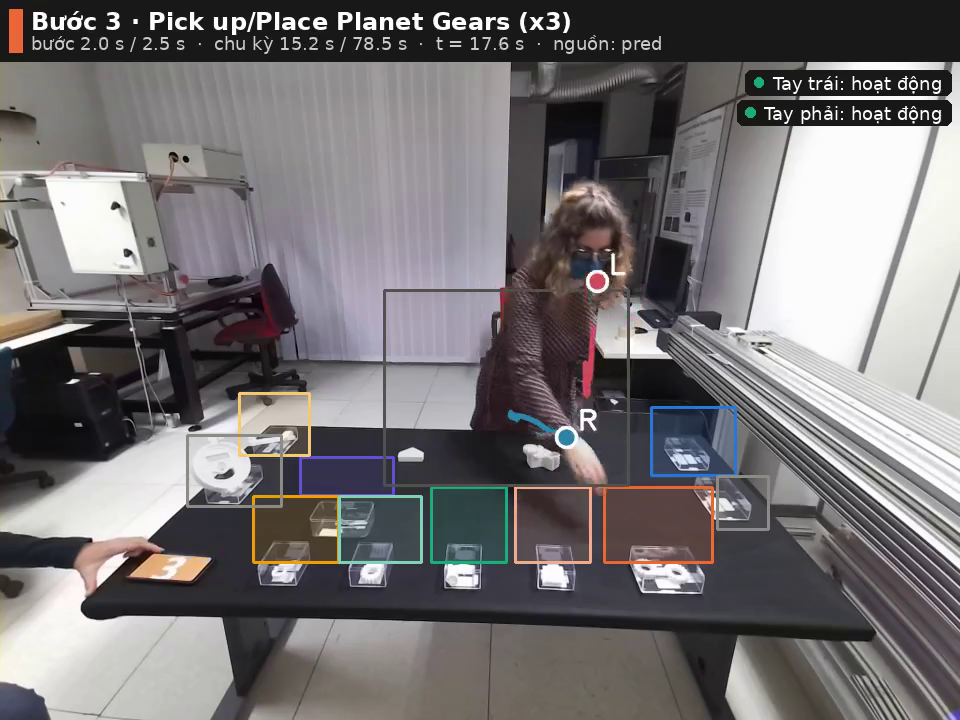
\includegraphics[width=0.8\textwidth]{frame_V001_step3.png}
  \caption{Video overlay sinh tự động: bước hiện tại, tiến độ trong bước và chu kỳ, trạng thái hai tay, zone và vệt cổ tay
  (U001\_V001, bước 3).}
  \label{fig:overlay}
\end{figure}

\subsection{Diễn giải LLM có kiểm chứng}
\label{subsec:exp_llm}
\Cref{tab:llm} tổng hợp tỷ lệ đạt validator qua các run.
Trong run có 4 phát hiện với RAG, Gemini 2.5 Flash đạt 3/4 ngay lần đầu.
Câu trả lời còn lại đạt sau một lần hỏi lại có phản hồi lỗi, nên tỷ lệ cuối là 100\%.
Mọi trích dẫn đều là \code{chunk\_id} có trong kho, và bảng tài liệu tham chiếu khớp hai chiều với các nhãn trong báo cáo.
Một bài học thực tế: ở lần chạy Gemini đầu tiên, câu ``phân vị 90'' bị đánh trượt oan
vì số 90 chỉ xuất hiện trong tên trường \code{dev\_p90\_deg}.
Sau khi bổ sung tập $\mathcal{N}(f)$ vào whitelist (\cref{eq:whitelist}), lỗi này không còn.
Validator không bắt được lỗi \textit{ngữ nghĩa}, ví dụ một con số có thật nhưng được gán sai ý.
Phần này vẫn cần kỹ sư IE duyệt.

\begin{table}[t]
\centering
\caption{Tỷ lệ đạt validator của tầng LLM}
\label{tab:llm}
\footnotesize
\setlength{\tabcolsep}{3pt}
\begin{adjustbox}{max width=\columnwidth}
\begin{tabular}{@{}llccc@{}}
\toprule
Provider / model & Ngữ cảnh & \#finding & Lần đầu & Sau retry \\
\midrule
Gemini 2.5 Flash & RAG (WI + KB) & 4 & 75\% & 100\% \\
Gemini 2.5 Flash & RAG & 1 & 100\% & 100\% \\
Gemini 3.8 Flash & KB/SOP tĩnh & 1 & 100\% & 100\% \\
Claude Sonnet 4.6 & RAG & \tbd & \tbd & \tbd \\
GPT-4.1 mini & RAG & \tbd & \tbd & \tbd \\
\bottomrule
\end{tabular}
\end{adjustbox}
\end{table}

\subsection{Thời gian chạy}
\label{subsec:exp_runtime}
Trên CPU, việc trích keypoint MediaPipe đạt khoảng 7{,}2--7{,}6\,fps, tức khoảng 6 phút cho mỗi video 80\,s.
Đây là bước chậm nhất, và kết quả được tái sử dụng giữa các run.
Các bước 02$\to$08 mất khoảng 8--9\,s cho 2 trial, chưa tính thời gian gọi LLM.
Render video overlay mất khoảng 2 phút mỗi video.
Suy luận MS-TCN: \todo{ms/video trên CPU}.
So với 2--4 giờ bấm giờ thủ công cho mỗi trạm, hệ thống cho số liệu của mọi chu kỳ đã quay,
thay vì chỉ vài chu kỳ được lấy mẫu.

\subsection{Thảo luận và giới hạn}
\label{subsec:limits}
\begin{itemize}
  \item \textbf{Quy mô dữ liệu.} Các số liệu đo được mới chỉ từ hai lần lắp của một người.
        Các chỉ số Mura giữa người và R1 cần nhiều trial và nhiều người hơn mới có ý nghĩa thống kê.
  \item \textbf{Phụ thuộc cấu hình trạm.} Zone được vẽ tay cho một camera cố định.
        Baseline quy tắc không tách được bước không có khay.
        Đặc trưng kp\_v1 dùng cả toạ độ tuyệt đối, nên một trạm hoặc camera mới cần dữ liệu có nhãn để train lại.
  \item \textbf{Đơn vị và hiệu chuẩn.} Quãng đường đang tính theo pixel (\code{px\_per\_cm}\,=\,null).
        Ngưỡng moving/still (120\,px/s) được chỉnh theo đồ thị tốc độ, chưa hiệu chuẩn hệ thống.
  \item \textbf{Muri 2D.} Góc chiếu phụ thuộc hướng camera, và tay trái chỉ đo được khoảng 25\% số frame.
        Chỉ số này chỉ dùng để sàng lọc.
  \item \textbf{Nhãn giả cho pose.} Fine-tune bằng skeleton Kinect có thể học cả sai số của Kinect.
\end{itemize}
